\section{이산 푸리에 변환 (DFT)}

\begin{frame}
    \frametitle{합성곱}
    \begin{block}{\textbf{합성곱(Convolution)}}
        두 벡터 \(\mathbf{a} = \left(a_0,\,\dots,\,a_{n-1}\right)\), \(\mathbf{b} = \left(b_0,\,\dots,\,b_{n-1}\right)\)\,에 대하여 이들의 \alert{합성곱} \(\mathbf{c} = \mathbf{a} \ast \mathbf{b}\)\,를
        \[
            c_i = \sum_{j = 0}^{i} \alert{a_{j} b_{i - j}} \qquad (i = 0,\,1\,\dots\,2n - 1)
        \]
        과 같이 정의한다.
    \end{block}

    \pause

    \begin{itemize}
        \item<2-> 다항식의 곱 형태와 동일한 모양: \alert{\(fg = f \ast g\)}
        \item<3-> 여전히 계산에는 \(\O(n^2)\)\,이 걸림
        \item<4-> Convolution\,을 빠르게... \textit{Fast Fourier Transform}?
    \end{itemize}
\end{frame}

\subsection{DFT}

\begin{frame}
    \frametitle{이산 푸리에 변환}
    \begin{block}{\textbf{Discrete Fourier Transform}}
        다항식 \(f = \left(a_0,\,\dots,\,a_{n-1}\right)\)\,의 \alert{이산 푸리에 변환}(DFT)을 다음과 같이 정의한다.
        \[
            \DFT(f) = \big(f(1),\, f(\omega),\, f(\omega^2),\, \dots\, f(\omega^{n-1})\big)
        \]
        단, \(\omega = \omega_n\) 이다.
    \end{block}

    \pause

    \begin{itemize}
        \item<2-> Roots of unity\,에 대해 \(f\)\,의 함숫값을 계산한 결과
        \item<3-> 결과는 \alert{벡터}
    \end{itemize}
\end{frame}

\begin{frame}
    \begin{theorem}
        다항식 \(f,\, g\)\,에 대하여 다음이 성립한다.
        \vspace*{-5px}
        \[
            \alert{\DFT(f \ast g) = \DFT(f) \cdot \DFT(g)}
        \]
        \vspace*{-15px}
    \end{theorem}

    \begin{itemize}
        \setlength{\itemsep}{1em}
        \item<2-> 우변의 \(\cdot\)\,은 성분별 곱 (component-wise product)
        \item<3-> \(f,\,g\)\,가 \(n\)\,차 다항식이면 \(fg\)\,는 \(2n\)\,차 다항식
        \item<4-> \(f,\,g\)\,를 \(2n\)\,차 다항식으로 간주하고 DFT\,를 계산
        \item<4-> \(f = (a_0,\,\dots,\,a_{n-1},\, \underbrace{0,\, \dots,\, 0}_{n\,\text{개}})\)
    \end{itemize}
\end{frame}


\begin{frame}
    \begin{proof}
        각 변의 \(k\)\,번째 성분만 비교하면 충분하다.
        \begin{center}
            (좌변) \(= (f \ast g)(\omega_{2n}^k) = (fg)(\omega_{2n}^k) = f(\omega_{2n}^k)g(\omega_{2n}^k) = \) (우변)
        \end{center}
    \end{proof}

    \pause

    \begin{corollary}
        다항식 \(f,\, g\)\,에 대하여 다음이 성립한다.
        \vspace*{-5px}
        \[
            \alert{f \ast g = \DFT\inv\left(\DFT(f) \cdot \DFT(g)\right)}
        \]
        \vspace*{-15px}
    \end{corollary}
\end{frame}

\subsection{Inverse DFT}

\begin{frame}
    \frametitle{DFT Matrix}
    \(\DFT(f)\)\,는 다음과 같이 표현 가능
    \[
        \DFT(f) = \underbrace{\begin{bmatrix}
                1      & 1              & 1                 & \cdots & 1                       \\
                1      & \omega         & \omega^2          & \cdots & \omega^{n - 1}          \\
                1      & \omega^2       & \omega^4          & \cdots & \omega^{2(n - 1)}       \\
                \vdots & \vdots         & \vdots            & \ddots & \vdots                  \\
                1      & \omega^{n - 1} & \omega^{2(n - 1)} & \cdots & \omega^{(n - 1)(n - 1)}
            \end{bmatrix}}_{W}
        \begin{bmatrix}
            a_0 \\ a_1 \\ a_2 \\ \vdots \\ a_{n - 1}
        \end{bmatrix} =
        \begin{bmatrix}
            f(1) \\ f(\omega) \\ f(\omega^2) \\ \vdots \\ f(\omega^{n - 1})
        \end{bmatrix}
    \]

    \pause

    \begin{itemize}
        \item<2-> \alert{DFT 행렬}: \(\ds W = \left(\omega^{ij}\right)_{n \times n}\) (0-based index)
        \item<3-> 역행렬만 찾아서 곱하면 Inverse DFT!
    \end{itemize}
\end{frame}

\begin{frame}
    \frametitle{DFT Matrix}
    \begin{theorem}
        DFT 행렬의 역행렬 \(W\inv\)\,는 다음과 같다.
        \[
            W\inv = \left(\frac{\omega^{-ij}}{n}\right)_{n\times n} = \frac{1}{n}\begin{bmatrix}
                1      & 1                 & 1                  & \cdots & 1                        \\
                1      & \omega^{-1}       & \omega^{-2}        & \cdots & \omega^{-(n - 1)}        \\
                1      & \omega^{-2}       & \omega^{-4}        & \cdots & \omega^{-2(n - 1)}       \\
                \vdots & \vdots            & \vdots             & \ddots & \vdots                   \\
                1      & \omega^{-(n - 1)} & \omega^{-2(n - 1)} & \cdots & \omega^{-(n - 1)(n - 1)}
            \end{bmatrix}
        \]
    \end{theorem}

    \pause

    \begin{proof}
        곱해보시라!
    \end{proof}
\end{frame}

\begin{frame}
    \frametitle{Inverse DFT}

    따라서, \(f = \DFT\inv(\DFT(f)) = W\inv \begin{bmatrix} f(1) \\ f(\omega) \\ \vdots \\ f(\omega^{n - 1}) \end{bmatrix}\)

    \pause
    \begin{theorem}
        다항식 \(f\)\,에 대하여 \(g = \DFT(f)\)\,라 하자. 그러면
        \[
            f = \DFT\inv(g) = \big(g(1),\, g(\omega^{-1}),\, g(\omega^{-2}),\, \dots,\, g(\omega^{-(n-1)})\big)
        \]
        이다.
    \end{theorem}
\end{frame}

\begin{frame}
    \frametitle{\(\DFT\) vs \(\DFT\inv\)}

    임의의 벡터 \((a_0,\, a_1,\, \dots,\, a_{n - 1})\)\,에 대하여 이를 다항식처럼 간주하고

    roots of unity\,에 대해
    \begin{columns}
        \column{0.5\textwidth}

        \begin{itemize}
            \item<2-> \(\DFT\): \alert{반시계} 방향으로 계산
        \end{itemize}
        \begin{center}
            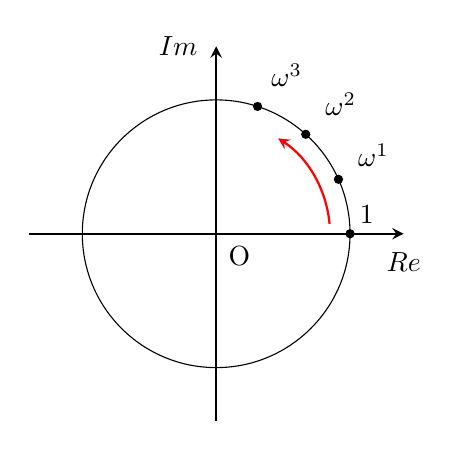
\begin{tikzpicture}[scale=1.7]
                \pgfmathsetmacro{\axislimit}{1.4}
                \pgfmathsetmacro{\n}{15}
                \node[below right=1pt] (origin) at (0,0) {\(\rm{O}\)};
                \draw [-stealth,thick] (-\axislimit, 0) -- (\axislimit, 0) node[below=3pt] {\(\mf{Re}\)};
                \draw [-stealth,thick] (0, -\axislimit) -- (0, \axislimit) node[left=3pt] {\(\mf{Im}\)};
                \draw (0, 0) circle (1);

                \only<2->{
                    \coordinate (one) at (1, 0);
                    \filldraw[fill=black] (one) circle (0.03) node[above right] {\(1\)};

                    \foreach \k in {1, 2, 3} {
                            \filldraw[fill=black] (360/\n * \k:1) circle (0.03);
                            \node[label=360/\n * \k - 5:\(\omega^{\k}\)] at (360/\n * \k:1) {};
                        }

                    \draw[-stealth,thick,color=red] (5:0.85) arc (5:57:0.85);
                }
            \end{tikzpicture}
        \end{center}

        \column{0.5\textwidth}
        \begin{itemize}
            \item<3-> \(\DFT\inv\): \alert{시계} 방향으로 계산
        \end{itemize}
        \begin{center}
            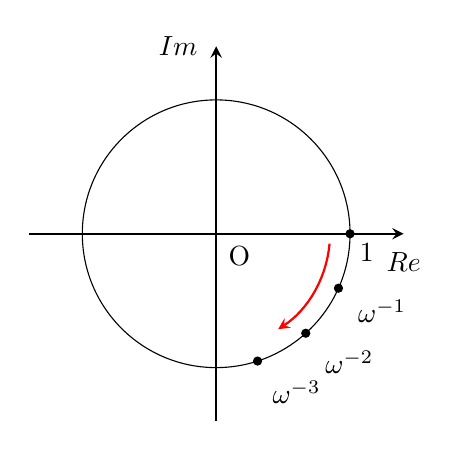
\begin{tikzpicture}[scale=1.7]
                \pgfmathsetmacro{\axislimit}{1.4}
                \pgfmathsetmacro{\n}{15}
                \node[below right=1pt] (origin) at (0,0) {\(\rm{O}\)};
                \draw [-stealth,thick] (-\axislimit, 0) -- (\axislimit, 0) node[below=3pt] {\(\mf{Re}\)};
                \draw [-stealth,thick] (0, -\axislimit) -- (0, \axislimit) node[left=3pt] {\(\mf{Im}\)};
                \draw (0, 0) circle (1);

                \only<3->{
                \coordinate (one) at (1, 0);
                \filldraw[fill=black] (one) circle (0.03) node[below right] {\(1\)};

                \foreach \k in {1, 2, 3} {
                        \filldraw[fill=black] (-360/\n * \k:1) circle (0.03);
                        \node[label=-360/\n * \k + 10:\(\omega^{-\k}\)] at (-360/\n * \k:1) {};
                    }

                \draw[-stealth,thick,color=red] (-5:0.85) arc (-5:-57:0.85);
                }
            \end{tikzpicture}
        \end{center}
    \end{columns}
\end{frame}
